\section{Object Re-identification Datasets}
\label{sec:ObjectReIDDatasets}

% ##############################################################################
\subsection{PKU VehicleID}
\label{ssec:DatasetPKUVehicleID}

The \datasetname{VehicleID} dataset~\cite{liu2016deepreldist} (web:~\cite{webpkuvehicledataset}) contains data captured during daytime by multiple real-world surveillance cameras distributed in a small city. There are $26\ 267$ vehicles ($221\ 763$ images in total). Each image is attached with an ID label corresponding to its identity in the real world (\figtext{}~\ref{fig:VehicleIDDataset}). In addition, there are manually labeled $10\ 319$ vehicles ($90\ 196$ images in total) of their vehicle model information (\ietext{} “MINI-cooper”, “Audi A6L”, “BWM 1 Series”, etc.). This dataset is usable thanks to the information about the model. We posit that at some point a hypothesis could be tested whether incorporating car model information into the machine learning model would improve its robustness. Nevertheless, only the front or rear view of the vehicle is available. This disadvantage is lessened by a reasonable number of training images. This dataset is also available only upon request and only for research purposes.

% ------------------------------------------------------------------------------
\begin{figure}[t]
    \centerline{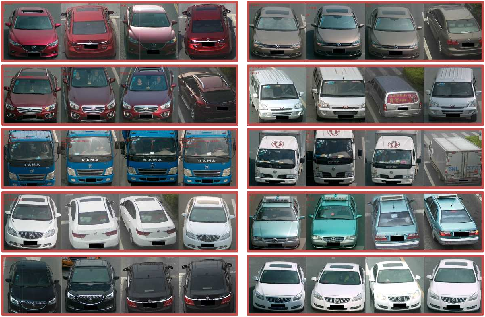
\includegraphics[width=0.5\linewidth]{figures/datasets/vehicleid_overview.pdf}}
    \caption[\datasetname{VehicleID} dataset]{Few samples from the \datasetname{VehicleID} dataset. Each vehicle has at least two images in the dataset, but only its front and rear view were obtained. \externalsrc{\cite{liu2016deepreldist}}}
    \label{fig:VehicleIDDataset}
\end{figure}
% ------------------------------------------------------------------------------

% ##############################################################################
\subsection{VeRI-776}
\label{ssec:DatasetVeRI776}

A large-scale benchmark dataset named \verisss{} (web:~\cite{webveridataset}) for vehicle \gls{reid} in the real-world urban surveillance scenario~\cite{liu2018provid} (\figtext{}~\ref{fig:VeRI776Dataset}). In our opinion, this dataset is one of the best available, and it already has been explored and served the purpose of training \gls{reid} models. The featured properties of this include the following important properties for training robust \gls{reid} models:

\begin{itemize}
    \item It contains over $50\ 000$ images of $776$ vehicles captured by $20$ cameras covering an $1\  \text{km}^2$ area in $24$ hours.
    \item The images were captured in a real-world unconstrained surveillance scene and labeled with varied attributes, \egtext{}, \glspl{bbox}, types, colors, and brands.
    \item Each vehicle is captured by at least $2$ up to $18$ cameras in different viewpoints, illuminations, resolutions, and occlusions.
    \item Data samples are also labeled with license plates and other spatio-temporal information, such as the \glspl{bbox} of plates with corresponding strings, the timestamps of vehicles, and the distances between neighboring cameras.
\end{itemize}

% ------------------------------------------------------------------------------
\begin{figure}[t]
    \centerline{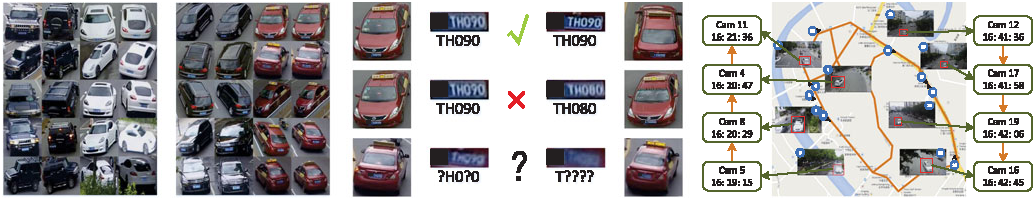
\includegraphics[width=\linewidth]{figures/datasets/veri776__overview.pdf}}
    \caption[\verisss{} dataset]{The properties of the \verisss{} dataset. Individual vehicles offer rich within-class differences in distinct viewpoints. At the same time, different but similar vehicles may have trivial inter-class differences. \externalsrc{\cite{liu2018provid}}}
    \label{fig:VeRI776Dataset}
\end{figure}
% ------------------------------------------------------------------------------
